\chapter{Hardware Model and Implementation}

This chapter details the hardware designed during this Master's thesis to accelerate neural network training. The current hardware implements both training and inference acceleration for the neural network architecture described in section \ref{net-arch}.
\todo[inline]{Refer to github, appendix, and project link}
\section{Specifications}
The hardware model was implemented using a ZedBoard. The ZedBoard is a development board equipped with a Zynq-7000 XC7Z020 SoC. The Zynq series has both a processing system and programmable logic, where the processing system is a ARM Cortex-A9 based processor (hereafter referred to as the ``PS'') and the programmable logic is an Artix-7 series FPGA. Bitstreams for the FPGA were generated using Vivado 2018.3 and PetaLinux boot images for the PS were created using Xilinx SDK. The hardware description language (HDL) code for the project was primarily written in SystemVerilog. The programs run on the PS were written in C.

\section{The Implemented Neural Network}\label{net-arch}
The classical MNIST handwritten digit dataset was chosen as the problem setting for the hardware model as a proof-of-concept. This problem has been chosen to verify the value in designing accelerators that take advantage of the finer-grained parallelism present in neural networks. The network consists of an input layer, 3 fully-connected layers, and a softmax output layer. The input layer is a 28$\times$28 grayscale image of a handwritten digit. The dimensions of the rest of the layers in the network are shown in table \ref{net-arch-table}. Layers whose name starts with FC are fully-connected layers.
 
\begin{table}
	\centering
	\begin{tabular}{|c| c| c|}
		\hline
		\textbf{Layer Name}	& \textbf{Input Size} & \textbf{Output Size}\\\hline
		FC0	& 784 (28$\times$28) & 98 \\\hline
		FC1 & 98 & 64 \\\hline
		FC2 & 64 & 10 \\\hline
		Softmax & 10 & 10\\\hline
	\end{tabular}
	\caption{The hidden and output layers in the implemented neural network}
	\label{net-arch-table}
\end{table}

Note that in this implementation, while biases are supported for forward computation, they are not used as the MNIST dataset is already fairly normalized. As such, the biases read are always 0 during the forward pass, and during the backward pass, no updates or gradients are calculated for the bias. Note that the gradient of the bias would just be the gradient of the neuron, unless the neuron had a ReLU activation function with negative net, so implementing this update would be trivial as all neuron gradients are already calculated. In addition, the current implementation only supports training with a batch size of 1.


\section{Design Goals}
There were a few key principles that guided the overall design process throughout the development of the hardware accelerator. A core tenet was to maintain the project such that in the future HDL could be generated for training a network of any architecture so long as the desired layer types had an implementation. As a result, all layers have been modularized and internal components are parameterized. Designing in a modular and parameterizable fashion also allows for quick and easy readjustments to the neural network architecture if needed.
\par 
In addition, optimal usage of resources available was prioritized. For example, the limiting FPGA resource was the amount of digital signal processing slices (DSPs). Therefore, the FPGA design optimized the distribution of DSPs over other resources as opposed to saving an extra Block RAM (BRAM) block. 

\section{Overall Architecture}
In the hardware model, both the Zynq's PS and the FPGA were used to facilitate a cohesive and efficient architecture to accelerate neural network computation. The overall system architecture can be seen in figure \ref{overall-arch}. 

Through memory-mapped I/O, the PS transfers neural net hyperparameters, training data, and control signals to the FPGA. The FPGA transfers training statistics and state data back to the PS. The interface is further described in sections \ref{az-com} and \ref{mmio-lay}.

Inside the FPGA, the neural network described in section \ref{net-arch} is implemented. Layers are connected in both forward and backward directions in order to support training. There are three types of primary modules in the top-level of the FPGA: fully-connected layers, interlayer activation buffers, and the softmax layer. In addition, there is a general control flow in the top-level with which all the primary modules interact.

\begin{figure}
	\centering 
	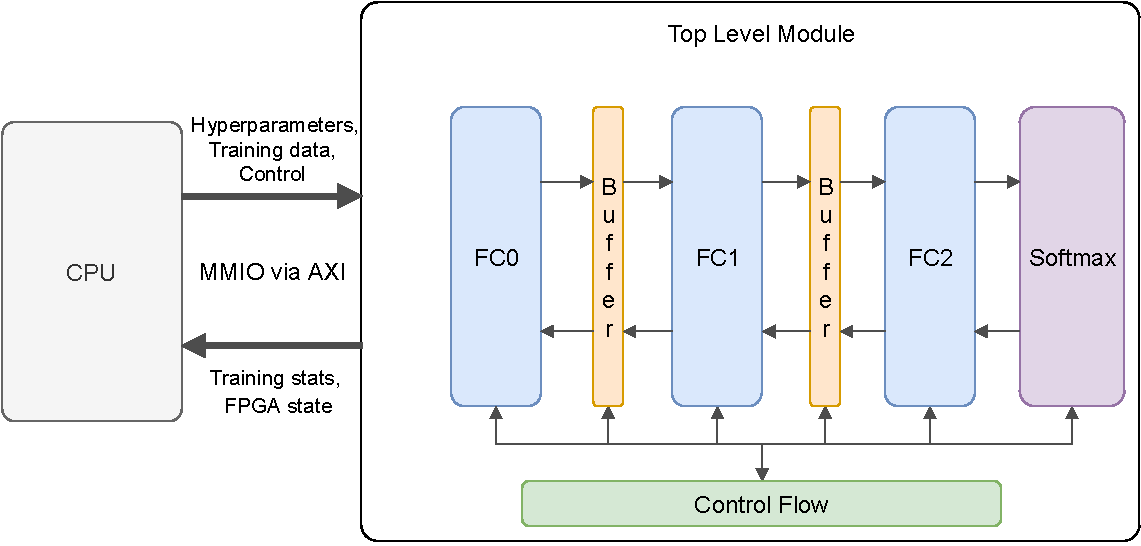
\includegraphics[width=\textwidth]{figures/overall_arch}
	\caption{Architecture of the hardware accelerator}\label{overall-arch}
\end{figure}


\section{Training Process}
The training process begins with the PS writing a 1 to the \texttt{start} register. This signals to the FPGA to start training whenever data becomes available. From the FPGA side, if the image in MMIO has ID equal to the FPGA's current image ID plus 1 (modulo image set size), then the image is ready.  Otherwise, the FPGA will wait for the next image to be written. This process is summed up in Figure \ref{ps-pl-training-process}. The FPGA loops back around to 0 once the image set size is reached. The image set size is assigned via MMIO. 

When the FPGA has processed the last image in the set during an epoch, the epoch counter is incremented and training stats will be available for the PS to read. If the epoch counter has reached the set number of training epochs, then training will stop, otherwise, the next training epoch will begin. 

\begin{figure}
	\centering 
	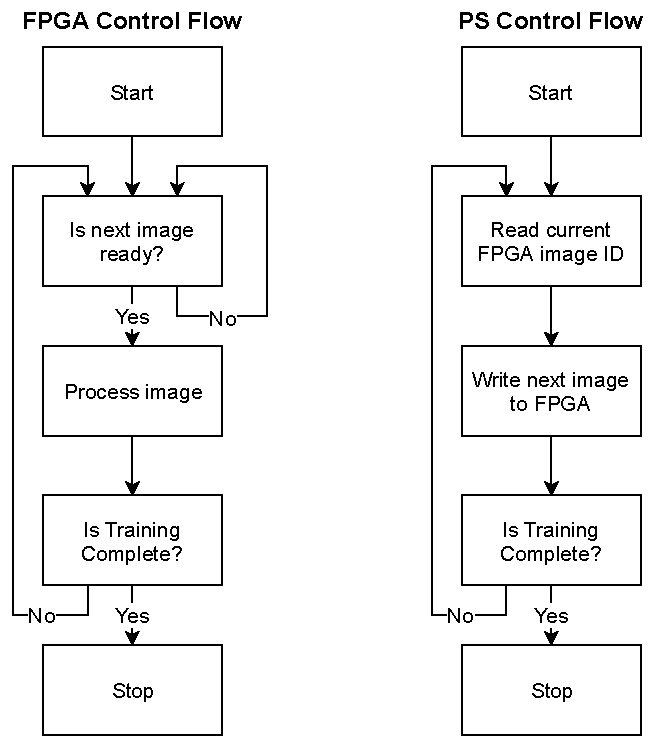
\includegraphics[width=3.5in]{figures/training_process_ps_pl}
	\caption{The high-level control flow of the training process}
	\label{ps-pl-training-process}
\end{figure}

\section{Computational Precision}
In this implementation, a bit-width of 18 was chosen for all weight gradients and activations. This value was chosen because the multiplication portion of DSP slices have an input multiplicands with bit widths of 25 and 18 \todo[inline]{cite dsp}. This thesis uses the Q number format to define precision types. For example, Q10.6 would mean that a 16-bit value has 10 integer bits and 6 fractional bits \cite{q-format}. For this accelerator, activations have a precision of Q6.12. Weights and weight gradients both have a precision of Q1.17. These values were chosen through experimental analysis of minimum and maximum activation, weight, and gradients values using the software model described in chapter \ref{ch-sw-model}.

\section{Module Architecture}
As mentioned in the design goal section, one of the tenets of this design was to allow for modularity and parameterization, such that changing a network architecture would not require too much work. As such, there are a few global parameters defined, such as the amount of bits specified for the fixed-point precision. There are also parameters defined for each of the fully-connected layers. These parameters can all be found in the \textit{sys\_defs.vh} file in the Appendix \todo[inline]{fpga appendix}, or on GitHub. 

\subsection{Fully-Connected Layers}
The fully-connected layer modules implement both forward and backward passes. The general architecture is shown in figure \ref{fc-arch}. As DSP slices are limited, both the forward and backward computational units make use of the same resources to compute multiplications, known as the kernel pool. There are 4 modes of computation in the fully-connected layer: forward pass, backpropagating neuron gradients, computing weight gradients, and updating the weights. Of these 4 modes of computation, all except updating the weights make use of the kernel pool. This is because updating the weights makes uses of bit shifting instead of multiplication to multiply gradients by the learning rate.
\begin{figure}
	\centering 
	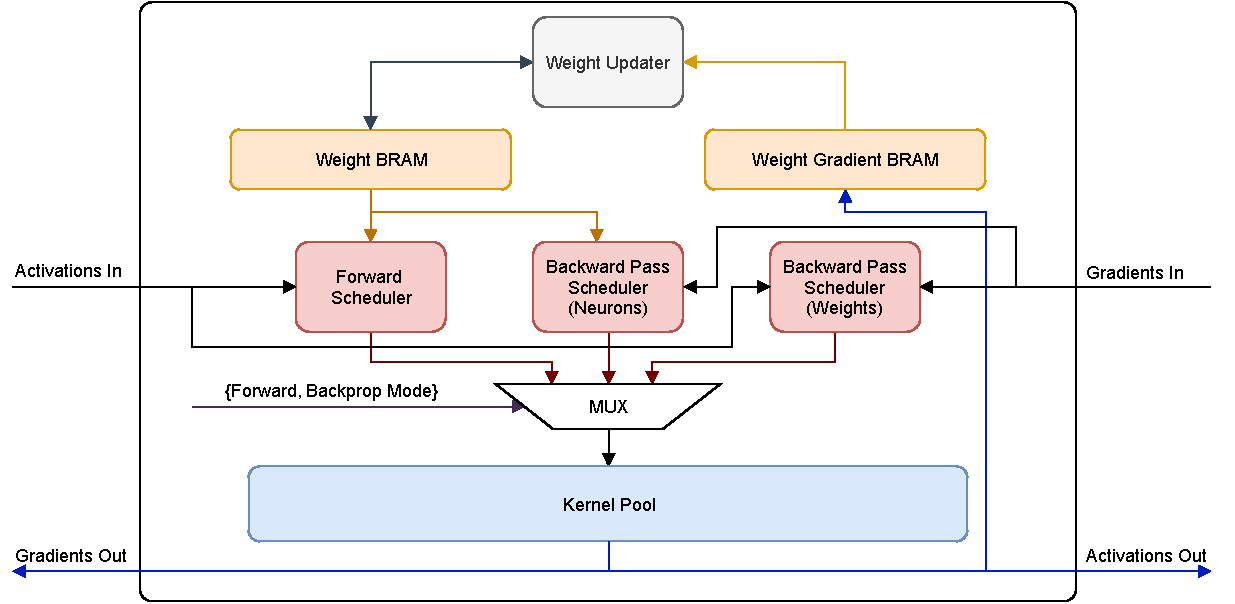
\includegraphics[width=\textwidth]{figures/fully_connected_arch}
	\caption{Architecture of the fully connected layer}\label{fc-arch}
\end{figure}

The forward pass multiplies weights and input activations to produce output activations. Backpropagating neuron gradients multiplies weights by current layer input gradients to produce previous layer gradients as output. The weight gradient computation mutliplies input activation from the forward pass by the current layer gradient, and then writing the computed gradient to the weight gradient BRAM. 

Since being flexible and modular was one of the design goals, all the fully-connected layers use the same kernel and scheduler modules, with different parameters in the instantiation.

\paragraph{Scheduling}
Each of the computational modes needs to have a scheduler to generate addresses to be read and guide the computation. For this, the a generalized scheduler module was implemented. The scheduler uses two pointers starting from the head and middle of the BRAM, and iterates through the entirety during the forward pass. Since the weight BRAMs of each layer are different, certain parameters are assigned for instantiations of the scheduler are also different.

\begin{lstlisting}[
caption={The instantiation of the scheduler for the FC1 layer}, label={sch_instant}, language=SystemVerilog, upquote=true]
fc_scheduler #(.ADDR(`FC1_ADDR), 
	.BIAS_ADDR(`FC1_BIAS_ADDR),
	.MID_PTR_OFFSET(`FC1_MID_PTR_OFFSET), 
	.FAN_IN(`FC1_FAN_IN)) 
	fc1_scheduler_i (
	//inputs
	.clk(clk),
	.rst(rst),
	.forward(forward),
	.valid_i(sch_valid_i),	
	//outputs
	.head_ptr(head_ptr),
	.mid_ptr(mid_ptr),
	.bias_ptr(bias_ptr),
	.has_bias(sch_has_bias)
);		
\end{lstlisting}
The instantiation of the scheduler shown in listing \ref{sch_instant} is similar across all the 3 fully connected layers, with only the parameters in the instantiations differing. The outputs are the pointers whose starting addresses are at the head and middle of the weight BRAM. In addition, there is a bias pointer and a signal to indicate if there is a bias.


\paragraph{Kernel}
The same kernel module is used in all the fully-connected layers. A high-level architecture of the computational kernel is provided in figure \ref{kernel-arch}. Note that saturation checking is not shown in the figure for simplicity, though it is implemented and verified. The scarcest computational resource in this FPGA architecture are the DSP slices, thus the kernel has been designed so that all required forms of multiplication are supported in the network. This is why there are 3 different outputs.

\begin{figure}
	\centering 
	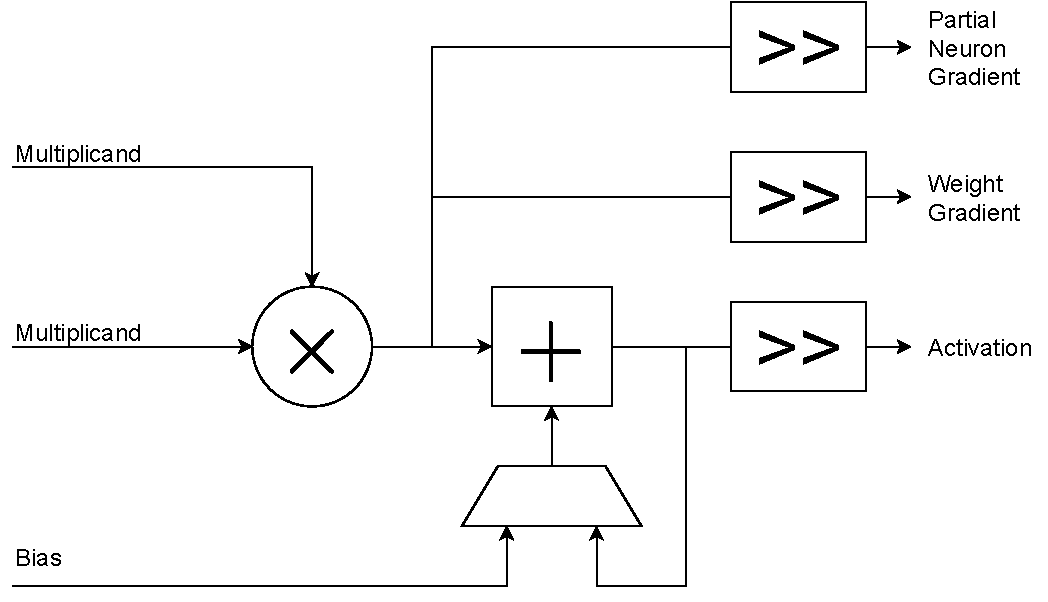
\includegraphics[width=5in]{figures/kernel_arch}
	\caption{Architecture of the kernel, saturation checking not shown.}\label{kernel-arch}
\end{figure}

From the figure, the top output is the neuron gradient. This multiplies a weight with a gradient. Multiplying two Q1.17 values results in a Q2.34 product, which must be checked for saturation in the top 2 bits and the bottom 17 bits must be truncated to obtain a Q1.17 output.

The middle output is the weight gradient. The weight gradients computation multiplies a gradient with an activation. As gradients are Q1.17 and activations are Q6.12, the output is Q7.29. To convert the resultant Q7.29 result to the desired Q1.17 format required for a weight gradient, the top 7 bits must be checked for saturation and the bottom 12 bits truncated. 

Finally, the bottom output is the net output calculated during the forward pass. This value becomes valid after performing $n$ MACs, where $n$ is the fan-in of a neuron. An input activation and corresponding weight are multiplied and added to either a bias or the running sum for the current in-progress net calculation. 

Since the forward pass multiplies Q6.12 activations by Q1.17, the multiplied result is 36-bits, Q7.29. Since for some layers fan-in can be quite large, extra precision is used during the accumulation phase. The accumulated sum uses 32 bits: Q6.26, thus the internal sum must be checked for saturation and truncation of the bottom 3 bits for each MAC. The conversion from the internal sum precision of Q6.26 to the net output of Q6.12 is a simple truncation of the bottom 14 bits.

With this amount of internal precision during the forward pass, truncation error during the internal summation is sufficiently minimized. This is because the largest fan-in in this network is 784 in the FC0 layer. For each internal MAC, the 27th fractional bit onward is truncated when converted from the product with precision Q7.29 to the internal sum precision of Q6.26. Assuming that the 27th bit equally probable to be 0 or 1, then the 27th bit is 1 approximately half of the time. This means that the average truncation per MAC is $0.5 \times 2^{-27} = 2^{-28}$. Given the 784 MACs of layer FC0, the expected truncation error is $784 \times 2^{-28} = 2.92\times{10^{-6}}$. The final truncation error from Q6.26 to Q6.12 truncates from the 13th fractional bit, resulting in an expected truncation error of $2^{-14} = 6.1\times10^{-5}$. Note that worst-case error is simply double the expected error, since it would assume that a 1-bit is truncated every time. Thus, truncation error from internal summation is expected to be more than 20 times less than the truncation to the 18-bit net output. Therefore, truncation error is successfully minimized during the internal summation of net computation during the forward pass.

The kernel is parameterized to support reuse in all the layers. The kernel has 2 parameters that are specified upon instantiation: neuron fan-in and the amount of bits needed to represent a neuron ID in the layer.

\paragraph{Weight Updates}
During the weight update phase, scaled weight gradients are added to the corresponding weight. This phase is implemented by iterating over the weight BRAM and weight gradient BRAM in the fully-connected layers. Scaling down the gradient by a learning rate is accomplished by using right bitshifts, which allows for efficient computation without any real sacrifice in training accuracy, as learning rates are generally arbitrary; frequently chosen as some power of 10.

One update phase takes two cycles. In the first cycle, the weights and their corresponding gradients for an address are read from the BRAMs. In the second cycle, the gradient is scaled down using bitshifting and added to the weight. The result is then written to the weight BRAM in the same cycle. The address will then be incremented and the process continues until all weights have been updated. The control logic is implemented by simply using a counter. The address to the BRAM contains all the bits except the bottom bit, so the address is incremented once every 2 cycles. The bottom bit of the counter is used to indicate the update phase and determine read and write enables on the BRAMs.

\subsubsection{Individual Fully-Connected Layer Implementation}
While the scheduler and kernels are the same across fully-connected layers, the weight BRAM specifications are not, since number of neurons, kernels and fan-in are different for each layer. For this reason, all fully-connected layers needed to have separate files defining them. If the weights and gradients were loaded and stored to from DRAM instead of BRAM, then the fully-connected layer could be parameterized.

\paragraph{Kernels Per Layer}
Given that the layers all have different amounts of MACs, the amount of computational kernels to allocate to each layer should be balanced to roughly even out the amount of cycles the computational phases require. There are 220 DSP slices available on the FPGA, and each kernel uses 1 DSP slice. In this design, 215 kernels were instantiated and the distribution is shown in table \ref{dsp-alloc}. The mathematical reasoning for this allocation is discussed in Chapter \ref{analysis}.
\begin{table}
	\centering
	\begin{tabular}{| c | c |}
		\hline
		\textbf{Layer} & \textbf{\# Kernels} \\\hline
		FC0 & 196 \\\hline 
		FC1 & 16 \\\hline 
		FC2 & 2 \\\hline	
		Total & 214 \\\hline	
	\end{tabular}
	\caption{Kernel allocation for the fully-connected layers in this implementation}
	\label{dsp-alloc}
\end{table}

\paragraph{Weight BRAM Initialization}
The BRAMs cannot be initialized with all 0 values as that devolve to being a linear classifier since all weights would have the same gradients, as explained in Chapter \ref{background}. Therefore, the weight BRAMs have been pre-initialized with values generated using He Initialization \cite{HeZR015}. The BRAMs are configured using Xilinx coefficient (COE) files. The initialization is performed using floating point, converted to Q1.17 binary format, and then written to a file in COE format using a python script. This script, \texttt{weight\_coeff.py} may be found in Appendix \todo[inline]{appendix for this} or in the \textit{misc} folder of the github repository.

\paragraph{BRAM Structure}
The memory storage and throughput requirements differed between the layers. As such, the weight and gradient BRAMs are organized differently. All the BRAMs use the true-dual port RAM configuration of the Xilinx Block Memory Generator IP Core, version 8.4. Each of the layers run be able to read 1 weight per kernel per cycle during computational steps to prevent kernels from idling. Note that the weight and gradient BRAMs are organized in the same way.

The FC0 layer has 196 kernels and 98 neurons, thus 196 weights need to be read per cycle.  This is accomplished by having two ports of width 98 weights wide. A weight is 18 bits, so the word length for each port is 1,764 bits wide. Furthermore, since the fan-in of each neuron is 784 ($28 \times 28$), there are 784 words in this BRAM. In total, the FC0 layer requires 49 36K BRAMs for the weights and the gradients each, or 98 total. The BRAM layout is shown in table \ref{fc0-bram}. The format for the weights listed in the word content is $w_{(i, j)}$, which meaning weight $i$ of neuron $j$.
\begin{table}
	\centering
	\begin{tabular}{|c|c|}
		\hline
		\textbf{Address} & \textbf{Word Content} \\\hline
		0 & $w_{(0, 0)}w_{(0, 1)}\cdots w_{(0, 96)}w_{(0, 97)}$\\
		1 & $w_{(1, 0)}w_{(1, 1)}\cdots w_{(1, 96)}w_{(1, 97)}$\\
		2 & $w_{(2, 0)}w_{(2, 1)}\cdots w_{(2, 96)}w_{(2, 97)}$\\
		$\cdots$ & $\cdots$ \\
		782 & $w_{(782, 0)}w_{(782, 1)}\cdots w_{(782, 96)}w_{(782, 97)}$\\
		783 & $w_{(783, 0)}w_{(783, 1)}\cdots w_{(783, 96)}w_{(783, 97)}$\\\hline
	\end{tabular}
	\caption{FC0 BRAM layout}	
	\label{fc0-bram}
\end{table}

The FC1 layer has 16 kernels and 64 neurons. 16 weights must be read each cycle to supply the neurons, so two ports of width 8 words are used. This means that the bitwidth of each port is 144 bits. The fan-in of each of the 64 neurons is 98, so there are 784 ($\frac{64\times98}{8}$) words in each BRAM for the weights and gradients. This results in needing eight 36K BRAMs for the FC1 layer. The first 98 words contain the weights for neurons 0-7. The subsequent 98 weights contain the weights for neurons 8-15. This continues through the entire contents of the BRAM, concluding with the last 98 words containing the weights for neurons 56-63. Since not every neuron is represented in every word, the memory layout is slightly different and shown in table \ref{fc1-bram}.

\begin{table}
	\centering
	\begin{tabular}{|c|c|}
		\hline
		\textbf{Address} & \textbf{Word Content} \\\hline
		0 & $w_{(0, 0)}w_{(0, 1)}\cdots w_{(0, 6)}w_{(0, 7)}$\\
		1 & $w_{(1, 0)}w_{(1, 1)}\cdots w_{(1, 6)}w_{(1, 7)}$\\
		$\cdots$ & $\cdots$ \\
		97 & $w_{(97, 0)}w_{(97, 1)}\cdots w_{(97, 6)}w_{(97, 7)}$\\
		& \\
		98 & $w_{(0, 8)}w_{(0, 9)}\cdots w_{(0, 14)}w_{(0, 15)}$\\		
		99 & $w_{(1, 8)}w_{(1, 9)}\cdots w_{(1, 14)}w_{(1, 15)}$\\
		$\cdots$ & $\cdots$ \\
		195 & $w_{(97, 8)}w_{(97, 9)}\cdots w_{(97, 14)}w_{(97, 15)}$\\	
		& \\	
		196 & $w_{(0, 16)}w_{(0, 17)}\cdots w_{(0, 22)}w_{(0, 23)}$\\		
		197 & $w_{(1, 16)}w_{(1, 17)}\cdots w_{(1, 22)}w_{(1, 23)}$\\
		$\cdots$ & $\cdots$ \\
		293 & $w_{(97, 16)}w_{(97, 17)}\cdots w_{(97, 22)}w_{(97, 23)}$\\	
		& \\
		$\cdots$ & $\cdots$ \\	
		& \\
		686 & $w_{(0, 56)}w_{(0, 57)}\cdots w_{(0, 62)}w_{(0, 63)}$\\		
		687 & $w_{(1, 56)}w_{(1, 57)}\cdots w_{(1, 62)}w_{(1, 63)}$\\
		$\cdots$ & $\cdots$ \\	
		783 & $w_{(97, 56)}w_{(97, 57)}\cdots w_{(97, 62)}w_{(97, 63)}$\\
		\hline
	\end{tabular}	
	\caption{FC1 BRAM layout}	
	\label{fc1-bram}
\end{table}

The FC2 layer is the smallest fully-connected layer in this hardware model, containing 10 neurons each with a fan-in of 64. There are 2 kernels, so each port on the BRAM has a word width equal to 1 weight, or 18 bits. The depth of the BRAM is 640, and can be entirely contained within one 36K BRAM. The layout is shown in table \ref{fc2-bram}.

\begin{table}
	\centering
	\begin{tabular}{|c|c|}
		\hline
		\textbf{Address} & \textbf{Word Content} \\\hline
		0 & $w_{(0, 0)}$\\
		1 & $w_{(0, 1)}$\\
		$\cdots$ & $\cdots$ \\			
		63 & $w_{(0, 63)}$\\
		& \\
		64 & $w_{(1, 0)}$ \\
		65 & $w_{(1, 1)}$ \\
		$\cdots$ & $\cdots$ \\	
		127 & $w_{(1, 63)}$\\
		& \\
		$\cdots$ & $\cdots$ \\	
		& \\ 
		576 & $w_{(9, 0)}$ \\
		577 & $w_{(9, 1)}$ \\
		$\cdots$ & $\cdots$ \\			
		639 & $w_{(9, 63)}$ \\
		\hline
	\end{tabular}	
	\caption{FC2 BRAM layout}	
	\label{fc2-bram}
\end{table}

\subsection{Interlayer Architecture}
In this implemented hardware model, activations stored in interlayer buffers are stored directly in flipflops. This is because there are only 98 activations from FC0 to FC1 and 64 from FC1 to FC2. This results in 162 18-bit activations being stored in interlayer activation buffers, far within the resource limitations of the FPGA.  The interlayer activation buffer module is also parameterized, so both buffers use the same SystemVerilog file. There are 5 parameters to be provided upon instantiation of the module, shown in table \ref{interlayer-arch-params}.

\begin{table}
	\centering
	\begin{tabularx}{\textwidth}{|l| X|}
		\hline
		\textbf{Parameter Name}	& \textbf{Brief Description}\\\hline
		\texttt{N\_KERNELS\_I} & 
		The width of the input write port. This is equivalent to the number of kernels of the previous layer. \\\hline
		
		\texttt{N\_KERNELS\_O} & 
		The width of the output read port. This is equivalent to the number of kernels in the next layer after the buffer.\\\hline
		
		\texttt{ID\_WIDTH} &
		The amount of bits needed to represent a neuron of the previous layer.\\\hline 
		
		\texttt{BUFF\_SIZE} &
		The amount of entries in the buffer. \\\hline 
		
		\texttt{LOOPS} &
		Amount of times the buffer needs to be looped through for the next layer after the buffer to finish its computation.
		\\\hline
	\end{tabularx}	
	\caption{Parameters required for instantiation of the interlayer activation buffer.}
	\label{interlayer-arch-params}
\end{table}

The architecture of the interlayer activation buffer is shown in figure \ref{interlayer-arch}. There is one write port which has a write width of \texttt{N\_KERNELS\_I} words. There are two read ports. The top one has a read width of \texttt{N\_KERNELS\_O} words and is used during the forward pass. The bottom one has a read width of 1 word and is used during the backward pass, particularly during the weight-gradient calculation phase.
\begin{figure}
	\centering 
	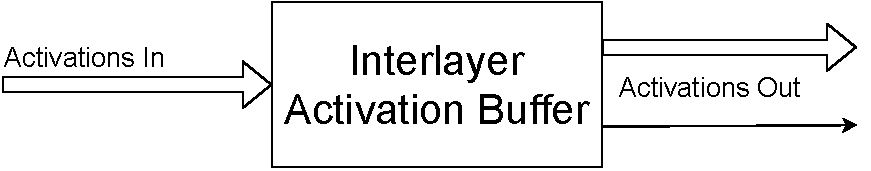
\includegraphics[width=\textwidth]{figures/interlayer_buffer}
	\caption{The interlayer activation buffer}\label{interlayer-arch}
\end{figure}

\subsection{Softmax Layer}
To implement training of the neural network, meaningful gradients needed to be calculated for the output layer neurons. Cross-entropy loss, one of the most popular loss functions in deep learning, was chosen for this network. As such, the softmax function (also described in Chapter \ref{background}) needed to be implemented. The softmax function is shown again in equation \ref{sm-func-impl} for convenience.
\begin{align}
\sigma(\mathbf{x})_i = \frac{e^{x_i}}{\Sigma_{j=1}^C e^{x_j}} \label{sm-func-impl}
\end{align}

The dataflow of the softmax layer is shown in figure \ref{softmax-arch}. The softmax layer has 10 inputs in this network for MNIST digit classification. This layer is fully pipelined, so while there is a relatively long latency, the computation can still be performed quickly. 

The implemented softmax function is also referred to as a numerically stable softmax. By subtracting a constant from the exponents, the final probabilities will not be affected. This is why the first step of the softmax layer is to subtract the maximum value input from all inputs. This then results in low, stable exponents being fed to the exponential function. 

Since there is no support for the exponential function using fixed-point inputs in the Xilinx IP core repository, logits are first converted to 32-bit floating point numbers. After this, the exponential function for each input is calculated. The $e^x$ core uses 1 DSP slice. The exponential function output is then converted from floating point back to fixed point. At this point, $e^x$ is known for all the inputs, so all the numerators required for $\sigma(\mathbf{x})_i$ are known. To calculate the denominator, these values must also be summed up, so this occurs in the next stage of the layer. Finally, the numerators are divided by this denominator to finish the softmax process of converting the outputs from logits to probabilities.
\begin{figure}
	\centering 
	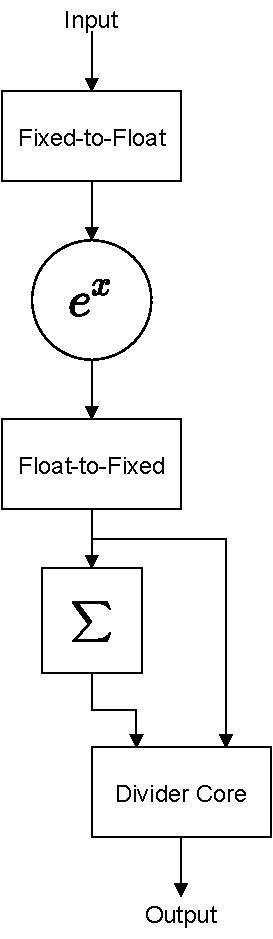
\includegraphics[height=\textheight]{figures/softmax}
	\caption{Architecture of the softmax layer}\label{softmax-arch}
\end{figure}


\section{PS -- FPGA Communication}\label{az-com}

The processing system and the FPGA communicate via an AXI4 bus. In this AXI bus, the PS is the master and the FPGA is the slave. 

\subsection{AXI Implementation for the PS}
From the PS side, communication is performed as shown by the highlighted red line in figure \ref{ps-con}. The AXI communication base address is 0x40000000 and spans until 0x7FFFFFFF. Having done this, by mapping a pointer to this location on \textit{/dev/mem}, data that is written to or read from addresses within this region of memory will invoke an AXI bus transaction. This was set up by adding the \textit{Zynq7 Processing System Version 5.5} IP core to a block diagram in Vivado, and defining an address range in the address editor as shown in Figure \ref{addr-editor}. 

\begin{figure}
	\centering 
	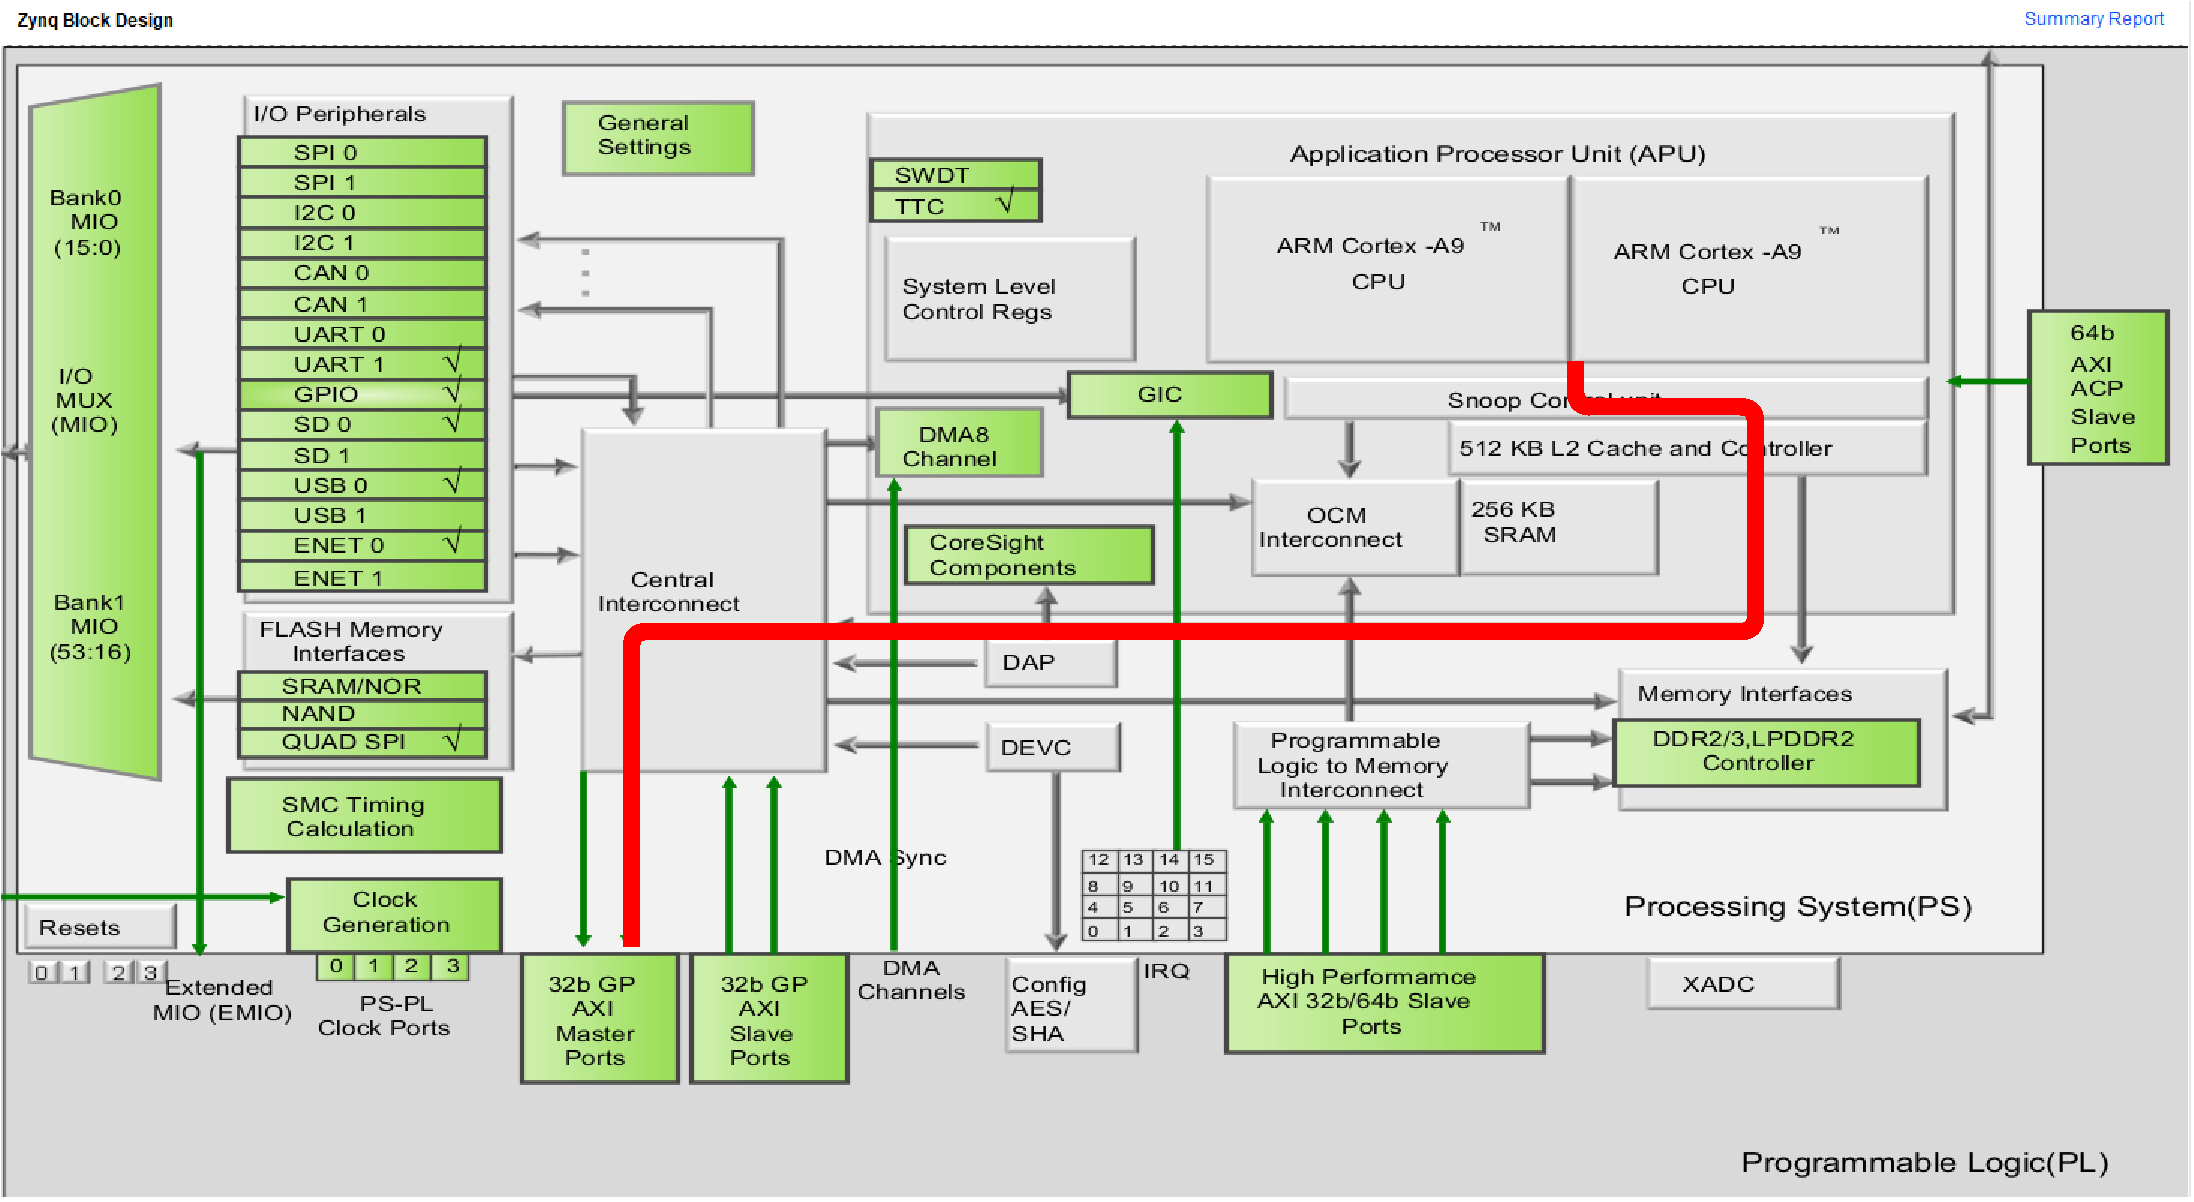
\includegraphics[width=\textwidth]{figures/ps-pl-conn}
	\caption{Communication from the PS to the FPGA}\label{ps-con}
\end{figure}

\begin{figure}
	\centering 
	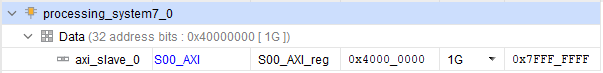
\includegraphics[width=\textwidth]{figures/address_editor}
	\caption{Specifying the Address Range for the AXI Bus}\label{addr-editor}
\end{figure}

Once the address range and Zynq IP core has been added to the block diagram, C code to run on the PS must be written. There are only 2 things that need to be done to be able to start performing AXI bus transactions. The first step is to create a file handle by opening \textit{/dev/mem} with the proper flags set. Then one only needs to memory map a pointer to this region. In the example shown in Listing \ref{mmap-c}, the pointer is of type volatile, because the order of reads and writes is critical during the training process when images are transferred to the FPGA.
\begin{lstlisting}[
caption={Code to allow the PS to perform AXI transactions with the FPGA}, label={mmap-c}, language=C, upquote=true]
int handle = open("/dev/mem", O_RDWR | O_SYNC); 
volatile ddr_data_t* ddr_ptr = mmap(NULL, 134217728, PROT_READ | PROT_WRITE, MAP_SHARED, handle, 0x40000000);
\end{lstlisting}

\subsection{AXI Implementation for the FPGA}
To implement the FPGA side of AXI commmunication, a block diagram to interface with the \textit{Zynq7 Processing System} was created. Next, a custom IP core was created using Vivado's base AXI4 slave and then customized to meet the design needs of the project. The block diagram was then completed as shown in Figure \ref{system-bd}. As can be seen, the Zynq's master AXI output is connected to an AXI interconnect which is then connected to the AXI slave port of the custom AXI module. Once the block diagram is complete, a wrapper for the block-diagram was generated and instantiated inside the top module of the design.

\begin{figure}
	\centering 
	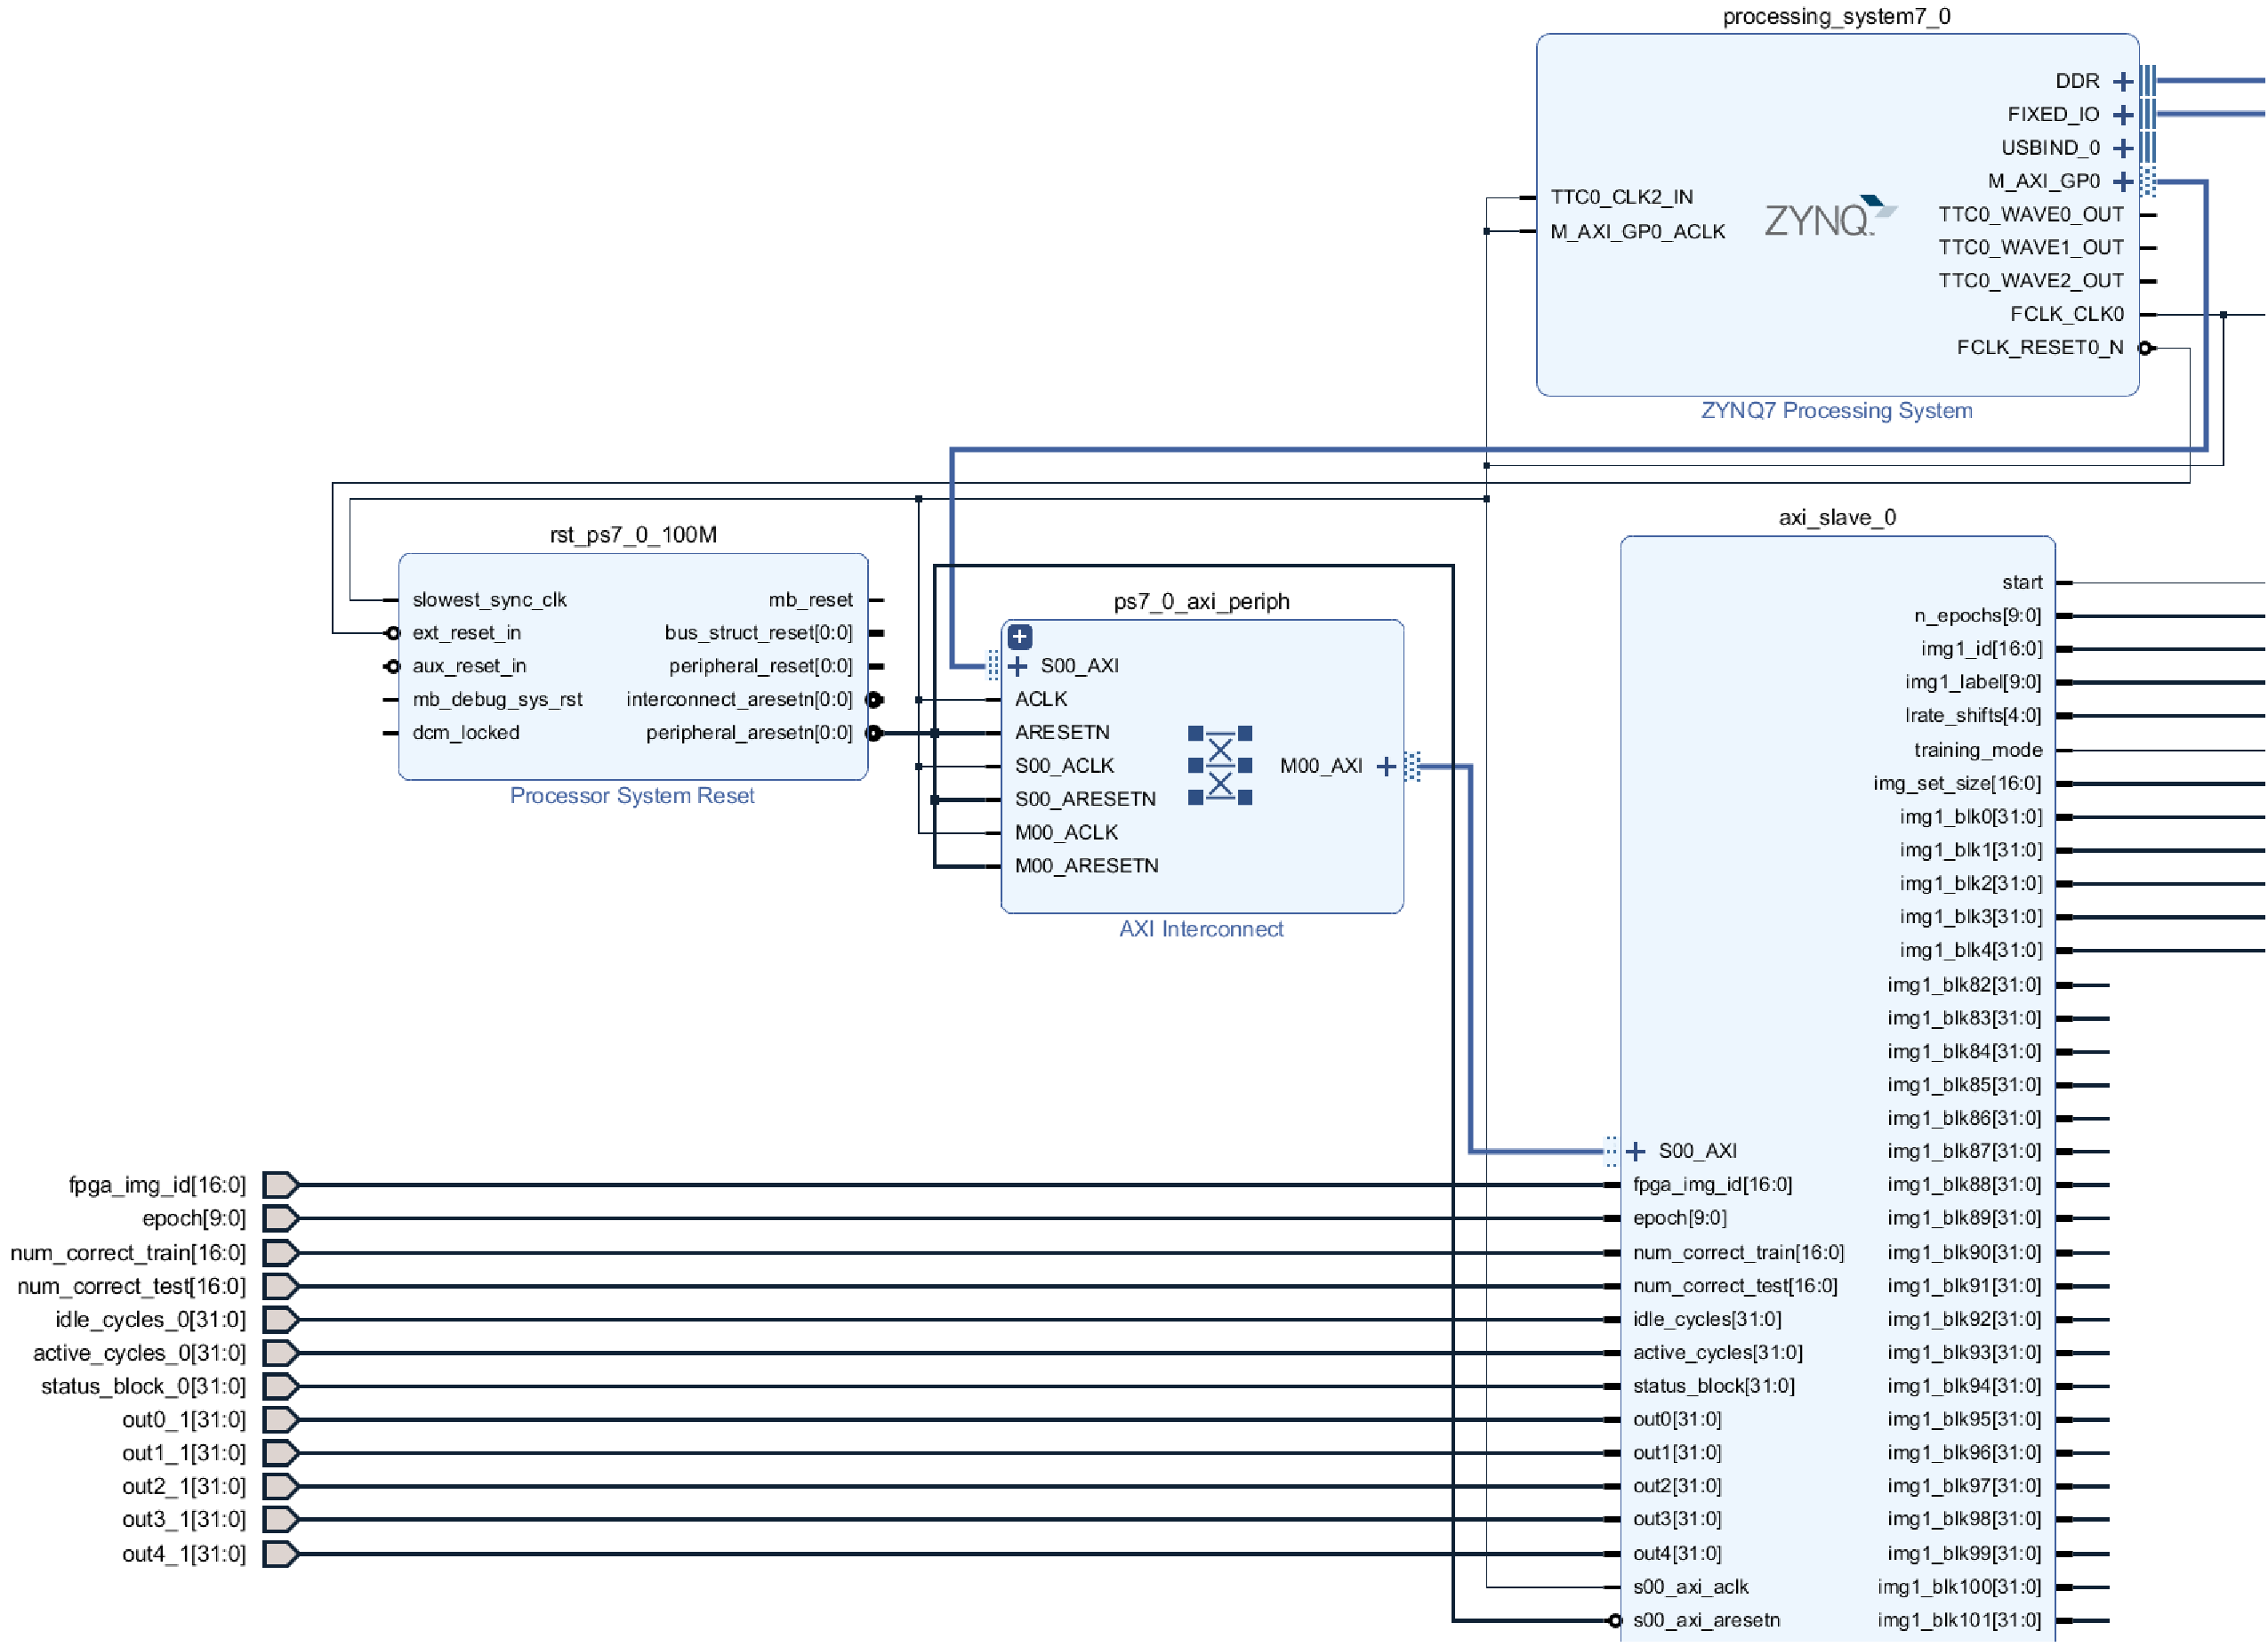
\includegraphics[width=\textwidth]{figures/fpga_axi_block}
	\caption{Block diagram to establish connection from the FPGA side to the AXI bus from the PS}\label{system-bd}
\end{figure}

The final part of the FPGA AXI implementation was to modify the generated AXI module. The module was generated in Verilog, so it differed slightly from the rest of the SystemVerilog project. It is also for this reason that there are 196 separate 32-bit registers to contain image data, since Verilog does not support 2D packed arrays as ports to modules. The Verilog code for implementing the memory map described in section \ref{mmio-lay} is included in Appendix \todo[inline]{verilog appendix}.

\subsection{Memory Map Layout}\label{mmio-lay}
The memory map may be extended easily by adding or modifying address definitions to the AXI slave connected to the PS in the FPGA. In the PS code, one only need modify the \texttt{ddr\_data} struct definition found in the C files of the PS source code. The memory map layout is defined in table \ref{tbl:mmio}. All addresses have a base address of 0x40000000. Note that values with addresses starting from 0x0 to 0x18 are registers written to by the FPGA. Values with addresses starting from 0x1C until 0x343 are written to by the PS. Output data from the FPGA is provided in the address range of 0x344 -- 0x358.
\begin{table}
	\centering
	\Large PS -- FPGA Memory Map \\\vspace{0.5em}
	\normalsize
	\begin{tabularx}{\textwidth}{|l| l| X|}
		\hline
		\textbf{Offset}	& \textbf{Name} & \textbf{Brief Description}\\\hline
		
		\texttt{0x0}	& 
		\texttt{fpga\_img\_id} & 
		The ID of the image that the FPGA is currently processing. \\\hline
		
		\texttt{0x4} &
		\texttt{epoch} &
		The current epoch in the FPGA \\\hline
		
		\texttt{0x8} &
		\texttt{num\_correct\_train} &
		The amount of correctly classified training images during the current epoch. \\\hline 
		
		\texttt{0xC} &
		\texttt{num\_correct\_test} &
		The amount of correct classified test images during the current epoch. \\\hline
		
		\texttt{0x10} &
		\texttt{idle\_cycles} &
		The amount of idle cycles in the FPGA since the start signal was received from the PS. An idle cycle is one in which none of the layers are performing any form of computation. \\\hline
		
		\texttt{0x14} &
		\texttt{active\_cycles} &
		The amount of active cycles in the FPGA since the start signal was received from the PS. An active cycle is one in which at least one of the layers is performing computations. \\\hline
		
		\texttt{0x18} &
		\texttt{status} &
		A 32-bit register with many different flags from the FPGA, such as the layer states, for example. \\\hline 
		
		\texttt{0x1C} &
		\texttt{start} &
		The start signal for training. \\\hline 
		
		\texttt{0x20} &
		\texttt{n\_epochs} &
		The number of epochs to train for in the FPGA \\\hline 
		
		\texttt{0x24} &
		\texttt{learning\_rate} &
		Value set to specify the amount of right shifts weight gradient should incur before updating a weight. \\\hline 
		
		\texttt{0x28} &
		\texttt{training\_mode} &
		Specifies whether the backward pass should be performed or not during computation.\\\hline
		
		\texttt{0x2C} &
		\texttt{img\_set\_size} &
		The size of the image set used during computation. \\\hline 
		
		\texttt{0x30} &
		\texttt{img\_label} &
		The label of the current image being computed. \\\hline 
		
		\texttt{0x34 -- 0x343} &
		\texttt{img} &
		Image data for the FPGA. \\\hline
		
		\texttt{0x344 -- 0x358} &
		\texttt{output} &
		Output data from the last layer in the FPGA, before the softmax function is performed, so they are still logits in this case.\\\hline		
	\end{tabularx}	
	\caption{Current memory map for communication between the PS and the FPGA.}
	\label{tbl:mmio}
\end{table}

\section{PetaLinux}
The boot image on the SD card has been modified to run Xilinx's PetaLinux. This was done by using the 2016.4 prebuilt PetaLinux image as a base from Xilinx's PetaLinux website \cite{petalinux}. The image has been slightly modified by changing the \textit{/etc/init.d/rcS} file to have the PS acquire a certain IP address and to mount the SD card to the filesystem. The \textit{BOOT.bin} for booting Petalinux on the PS is created by writing a first stage bootloader \textit{elf} file created by the Xilinx SDK for the Vivado project, the bitstream generated by Vivado, and the \textit{u-boot.elf} file from the 2016.4 PetaLinux image. The boot image is created by using Xilinx SDK's ``Create Boot Image'' utility. Aside from these changes to the 2016.4 SD card image, the other files in the image are not changed.

\paragraph{Cross-Compiling for PetaLinux}
Since the PS is an ARM-based processor, all C code for this project must be cross-compiled before it can be run on the PS. This is done by using the Linaro cross-compiling toolchain. A C file may be compiled to run on the PS using the below command.
\begin{lstlisting}
> arm-linux-gnueabi-gcc <source_file> -o <executable>
\end{lstlisting}

\section{Project Structure}
\todo[inline]{Ask if this is actually something I should do. Probably more documentation-y than implementation}